\chapter{Evaluation}\label{ch:evaluation}

Due to there being three major stages to the evaluation (preprocessing, training/testing, translating) as explained in Chapter~\ref{ch:methods}, and these three stages having different bottlenecks, not all experiments were run on the same computers. Both the preprocessing and translating stages require the reading of the entire data set file, making it very RAM intensive. They also only require CPU work, shifting the bottleneck to the CPU after reading the file. Preprocessing also allows for CPU parallelization, making more CPUs a very good thing to have. As such the first and third stages are run on a computer with 1.5TB of ram and 16 Intel Xeon E5--2630v3 CPUs running at 2.40GHz with 32 threads.The training/testing stage however, is a very GPU intensive task. Due to parallelization being highly effective for this task, as explained in Chapter~\ref{ch:methods}, the amount of GPUs is very influential for this task, offering close to linear performance improvements, the second task was ran on a computer with 1TB of ram, 20 Intel Xeon E5--2650v3 CPUs running at 2.30GHz with 40 threads and 16 NVIDIA Tesla K80 GPUs each with 11.5GB of memory. 

Due to the size of the data set and the limited amount of time, the decision was made to use only 5\% of the data set for plots/results, as such the percentage that has been used will be 5\% in the following results unless states otherwise. Keep in mind that this means the first 5\% of the file, not 5\% of users. This means that approximately 3 days of data is being used. This causes many users to not have enough actions to pass the 150 actions baseline. Increasing this percentage will not only increase the actions for existing users (causing an exponential increase in work required) but also introduces new users, also leading to an exponential increase in work. 

In order to get an idea of how the percentage of the data set takes with the time commands take to run, a percentage of 0.1\% has occasionally also been used. Doing preprocessing took 38 seconds for 0.1\% of the data while it took 40m16s for 5\% of the data, both using 10 CPUs. A very rough estimate puts the duration of preprocessing the entire data set at about 40 hours also using 10 CPUs. Doing the training/testing stage took 1h51m using 16 GPUs on 0.1\% of the data set, while 1\% took about 10 hours and 5\% of the data took 62h0m36s, giving a rough estimate of 2000 hours for 100\% of the data set. The anomaly translation part generally only takes roughly 2 and a half hours, not varying much between data set sizes as all users need to be iterated through regardless and no other heavy CPU work is being done. The biggest time sink for this part is loading the data set file itself at about 2h15m. Putting this all together, the entire process takes 65h10m52s for 5\% of the data. The 5\% data set contains 50,276,292 actions, meaning the network can handle about 214 actions per second, making this very fit for real-time anomaly detection. The actual testing stage (without training) takes even shorter, generally only taking a few seconds per user for all their actions, which would make a network that doesn't continue learning after the initial training even more feasible to run.

\begin{figure}
	\begin{center}
		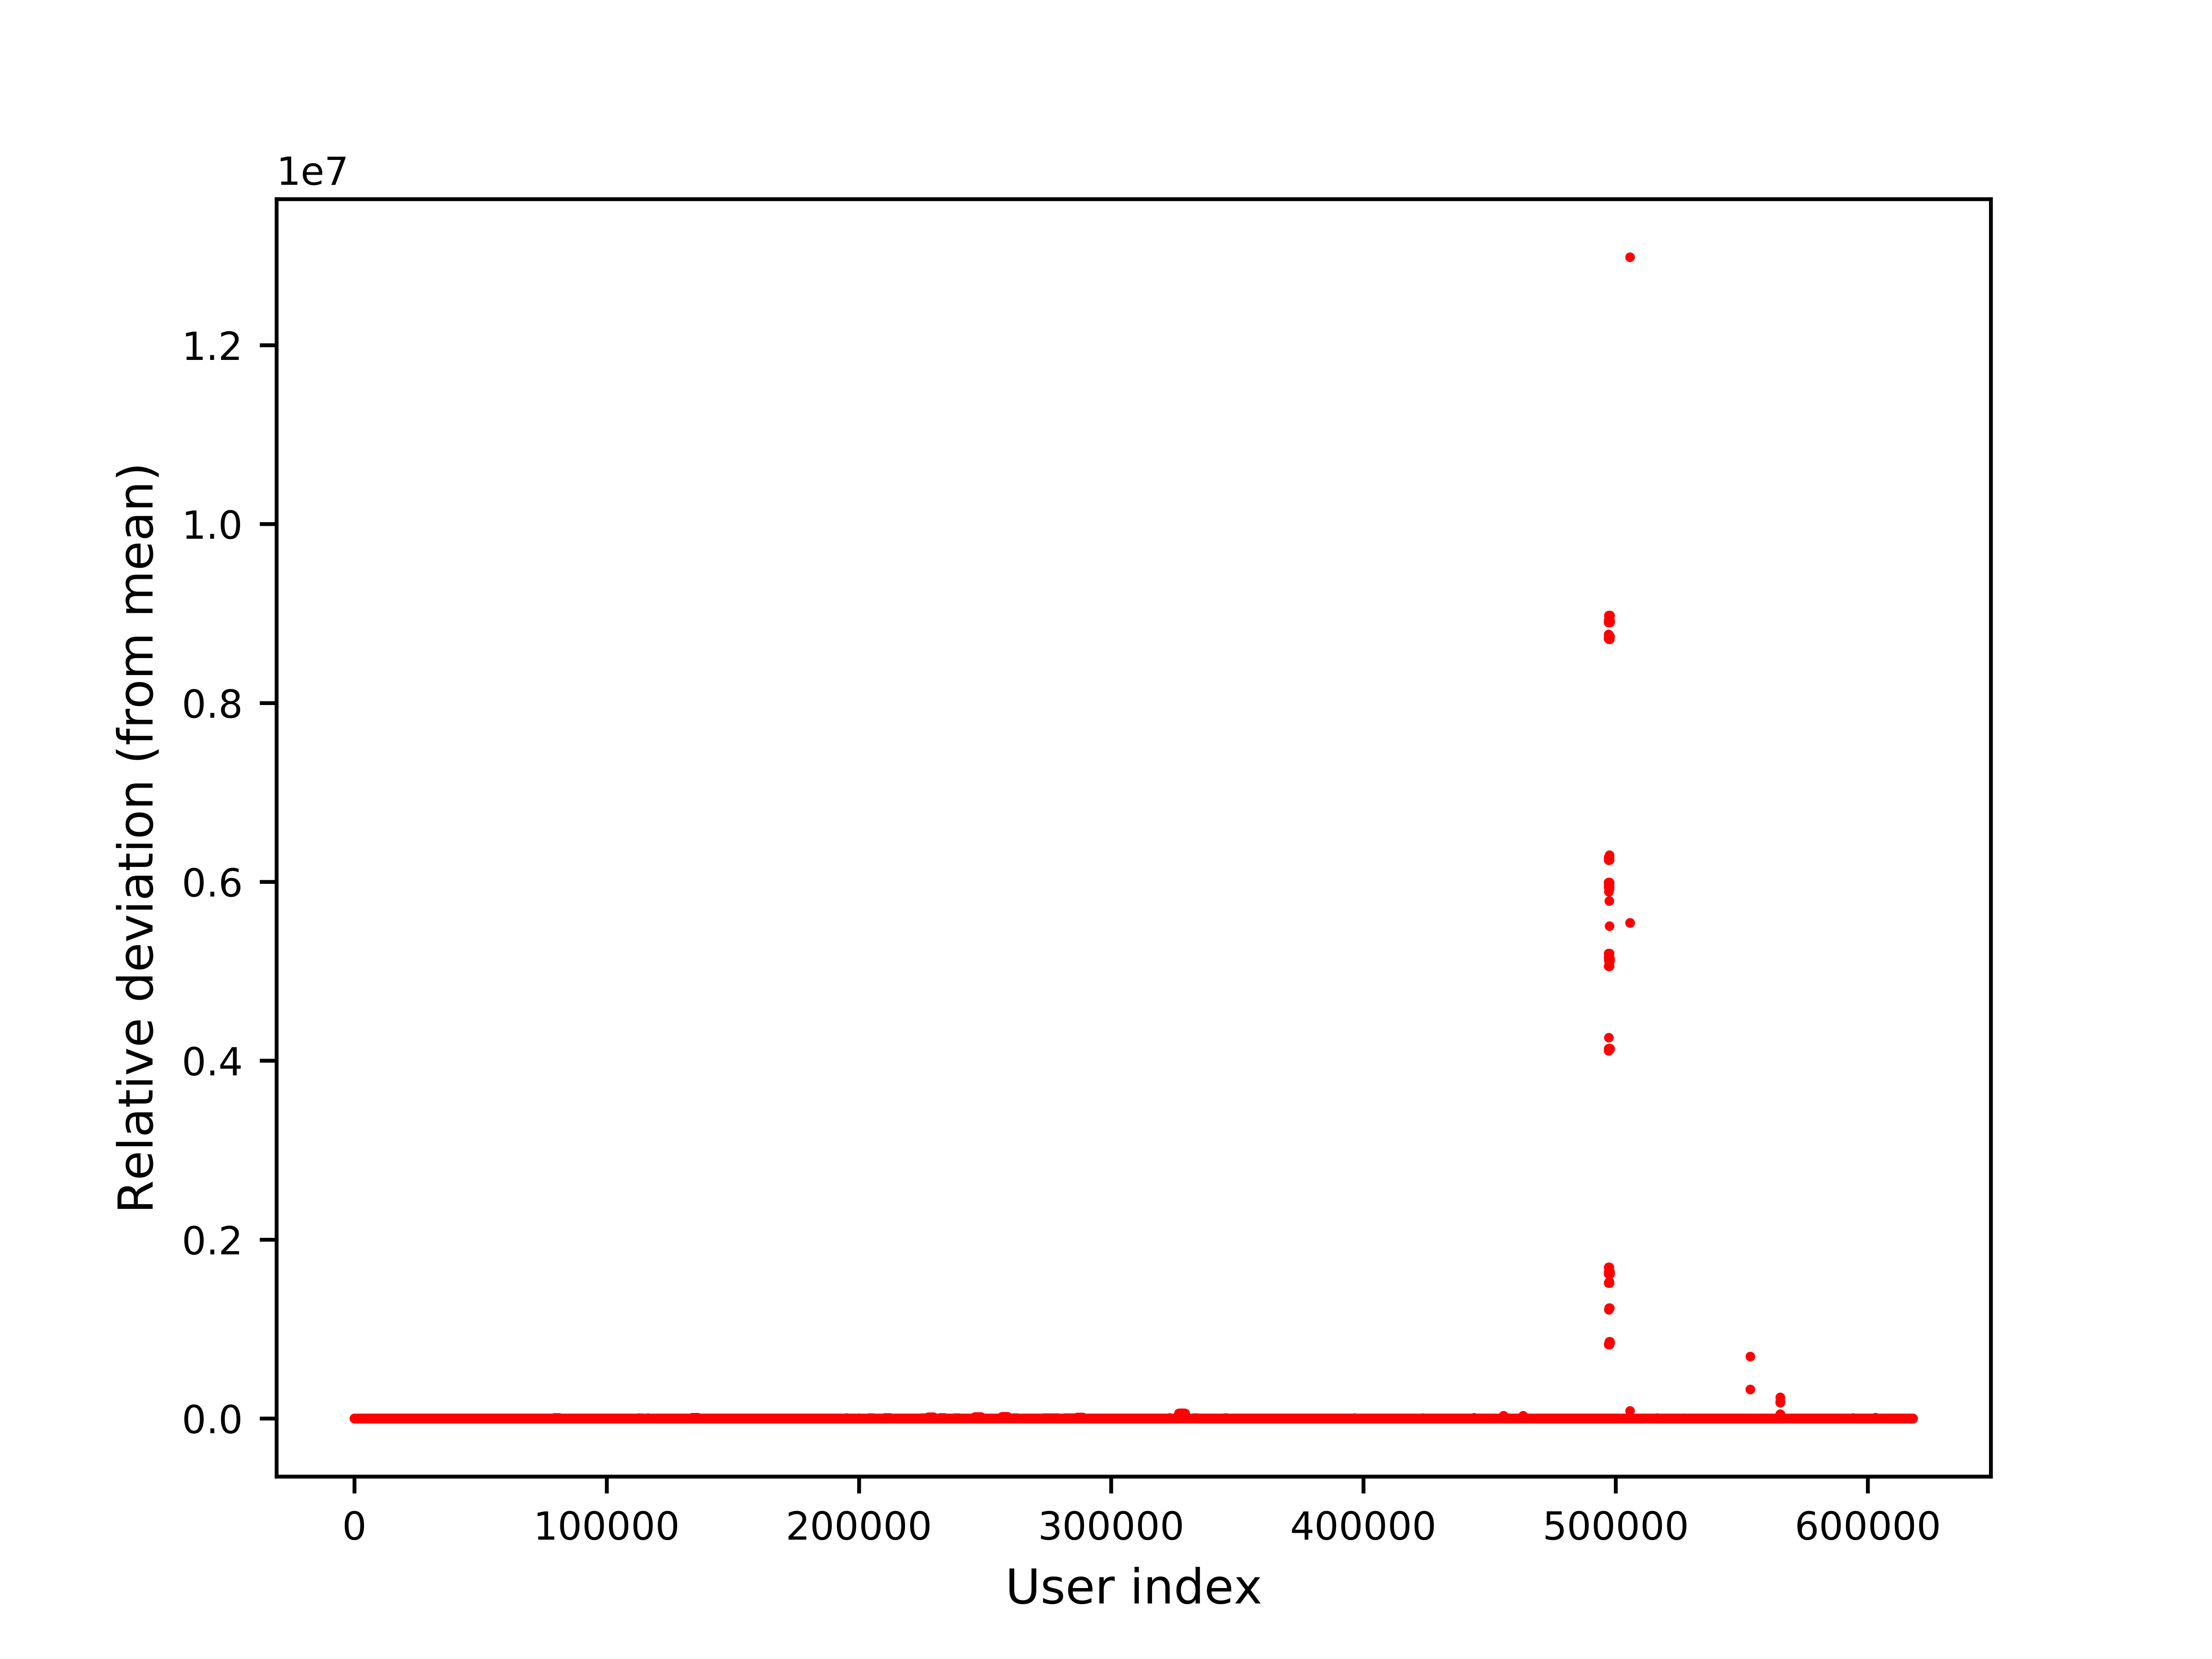
\includegraphics[scale=0.1]{evaluation/all_deviations}
	\end{center}
	\caption{All deviations from the IQR.~\label{fig:iqr_scale}}
\end{figure}

In figure~\ref{fig:iqr_scale}, the deviations from the IQR can be seen for all actions. This deviation is equal to the distance from the IQR calculated by the following formula, where x is equal to that action's loss value:

\( deviation = (x - Q3) / IQR \)

This leads to a deviation for which any value greater than 1.5 is an outlier (as discussed in Chapter~\ref{sec:methods:testing}). As can be seen in~\ref{fig:iqr_scale}, there are quite a number of outliers, some of which having outliers that fall far beyond the cutoff value of 1.5. From this we can conclude that at least some anomalies are being found. 

\begin{figure}
	\begin{center}
		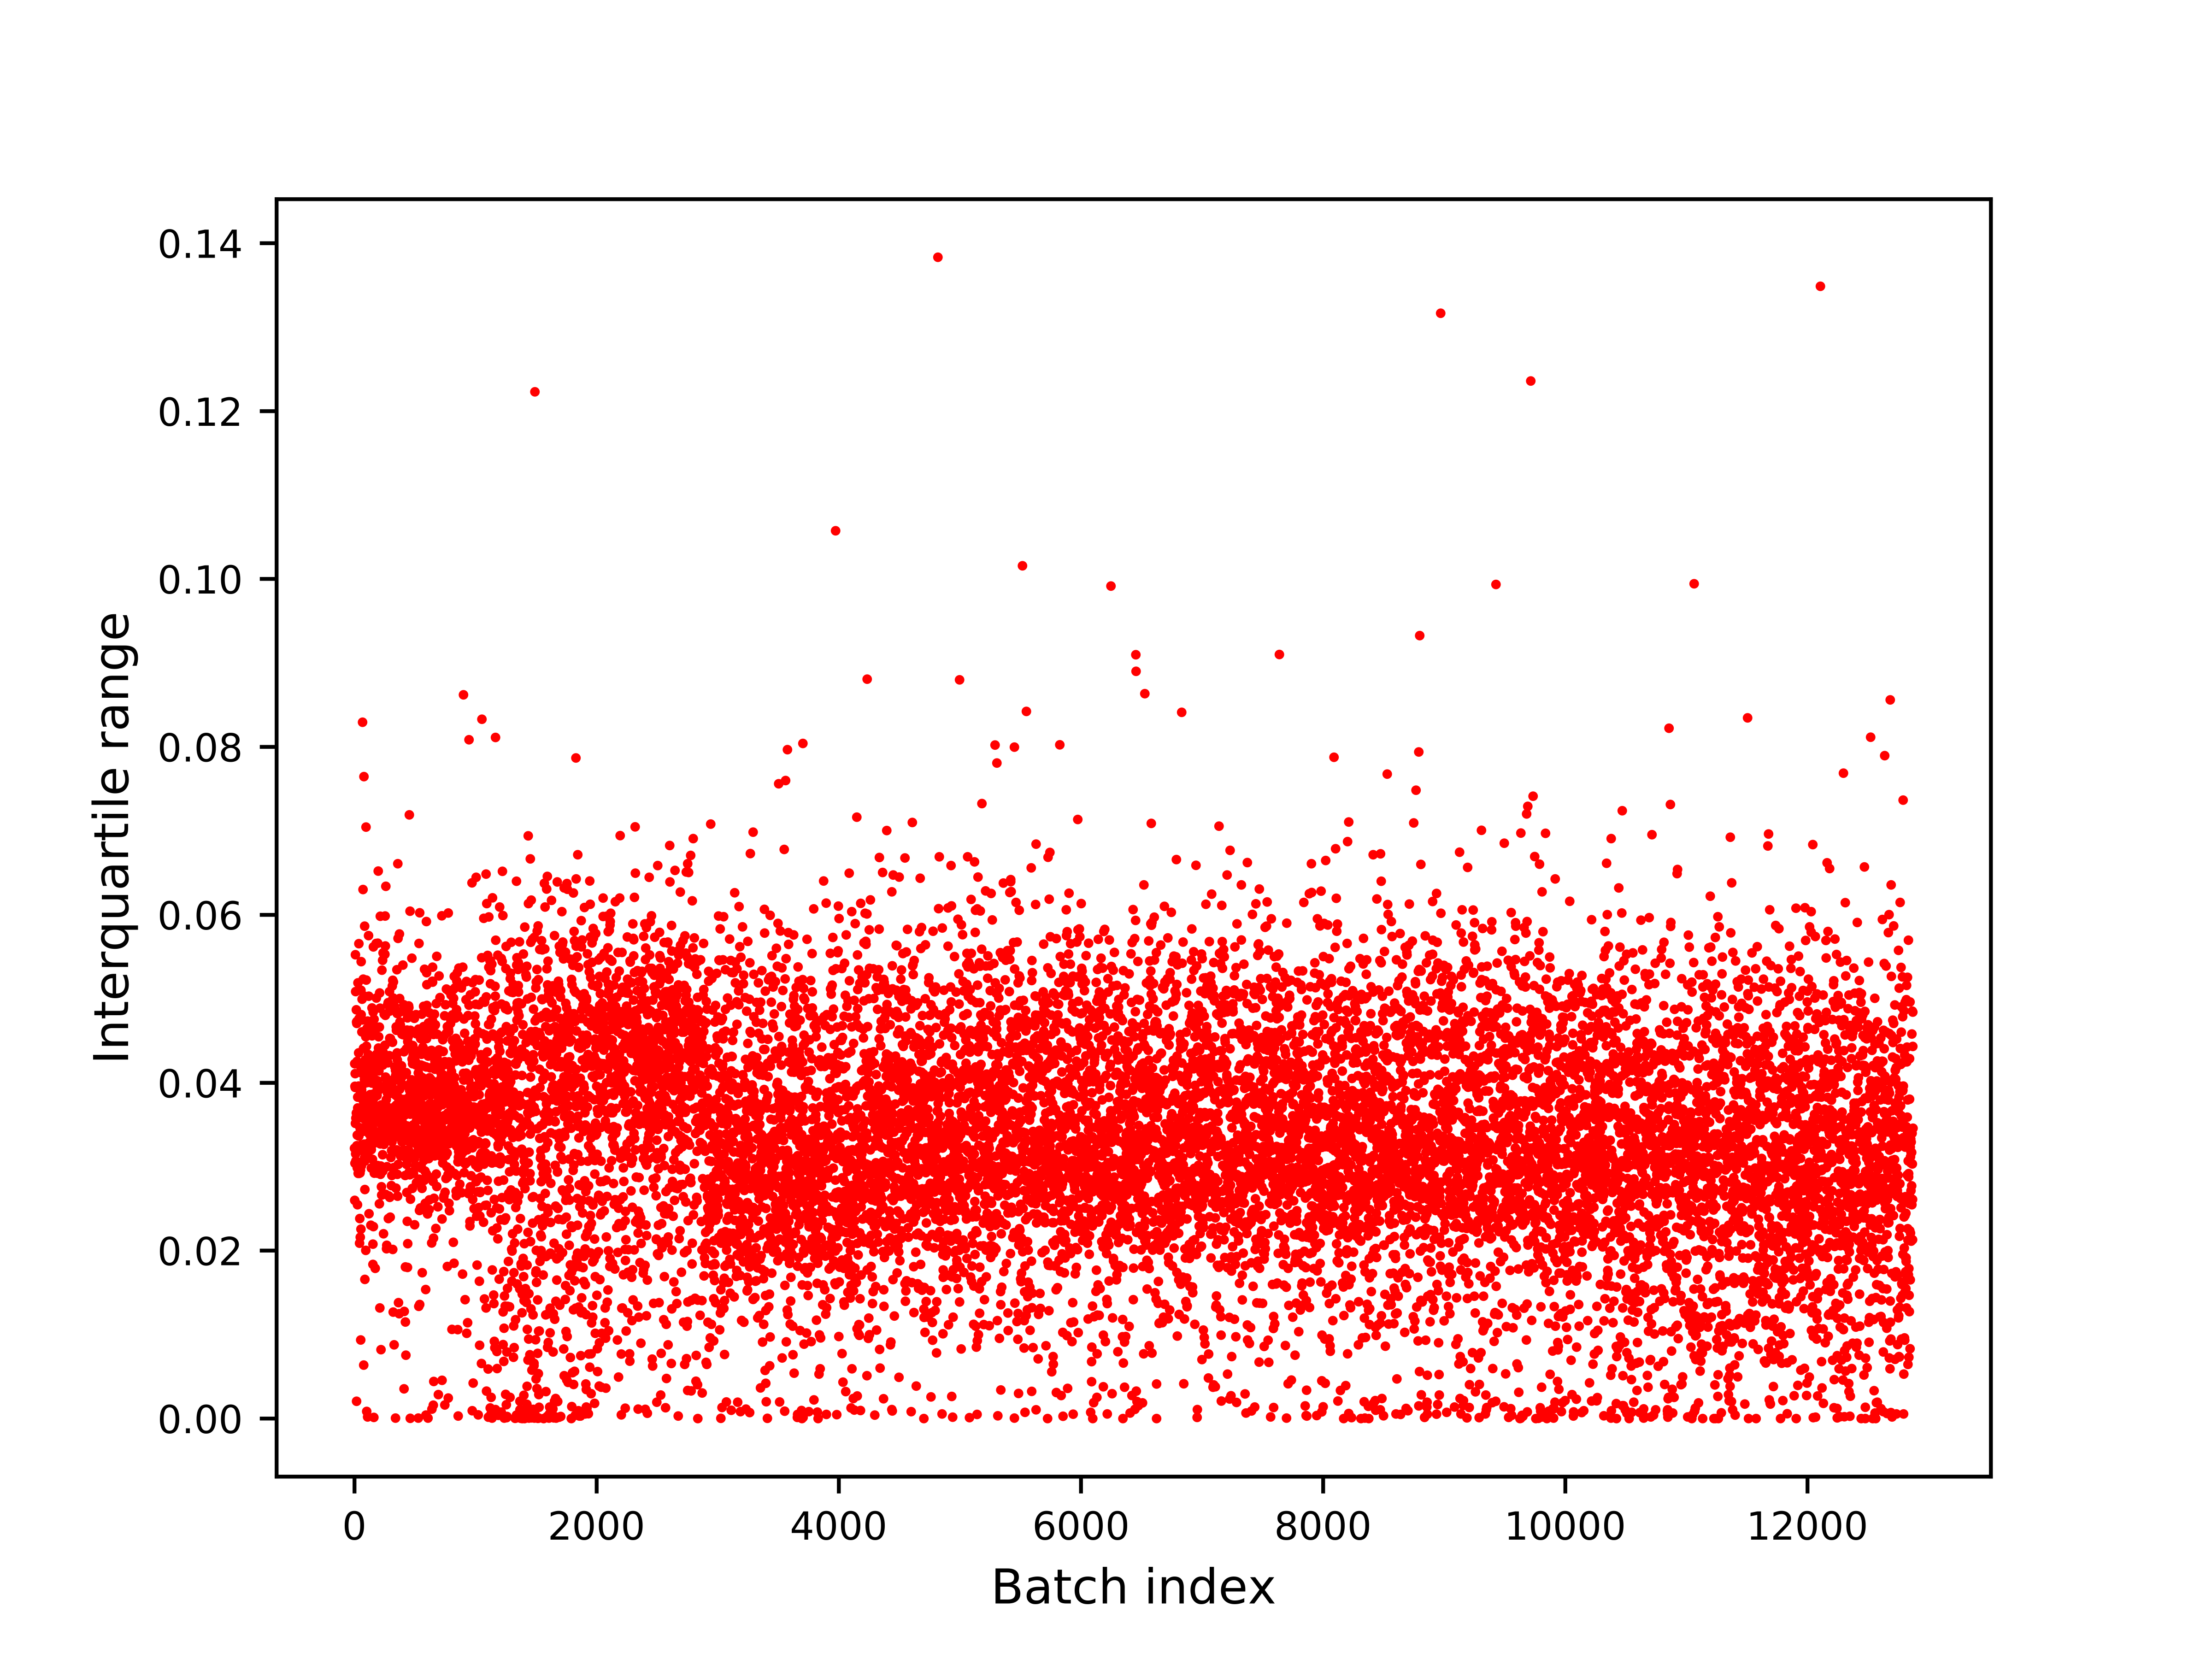
\includegraphics[scale=0.1]{evaluation/iqrs}
	\end{center}
	\caption{All IQR values.~\label{fig:iqrs}}
\end{figure}

As can be seen in figure~\ref{fig:iqrs}, the IQRs tend to be fairly close to each other, meaning the mean losses are close to each other as well. This shows that the network is relatively successful at modeling user behavior, as the difference between the expected and actual action calculated by the loss function shows few big spikes. A network that is unsuccessful at this would have inconsistent IQRs as the losses would fluctuate more from user to user and would show higher values indicating bad predictions.

\begin{figure}
	\begin{center}
		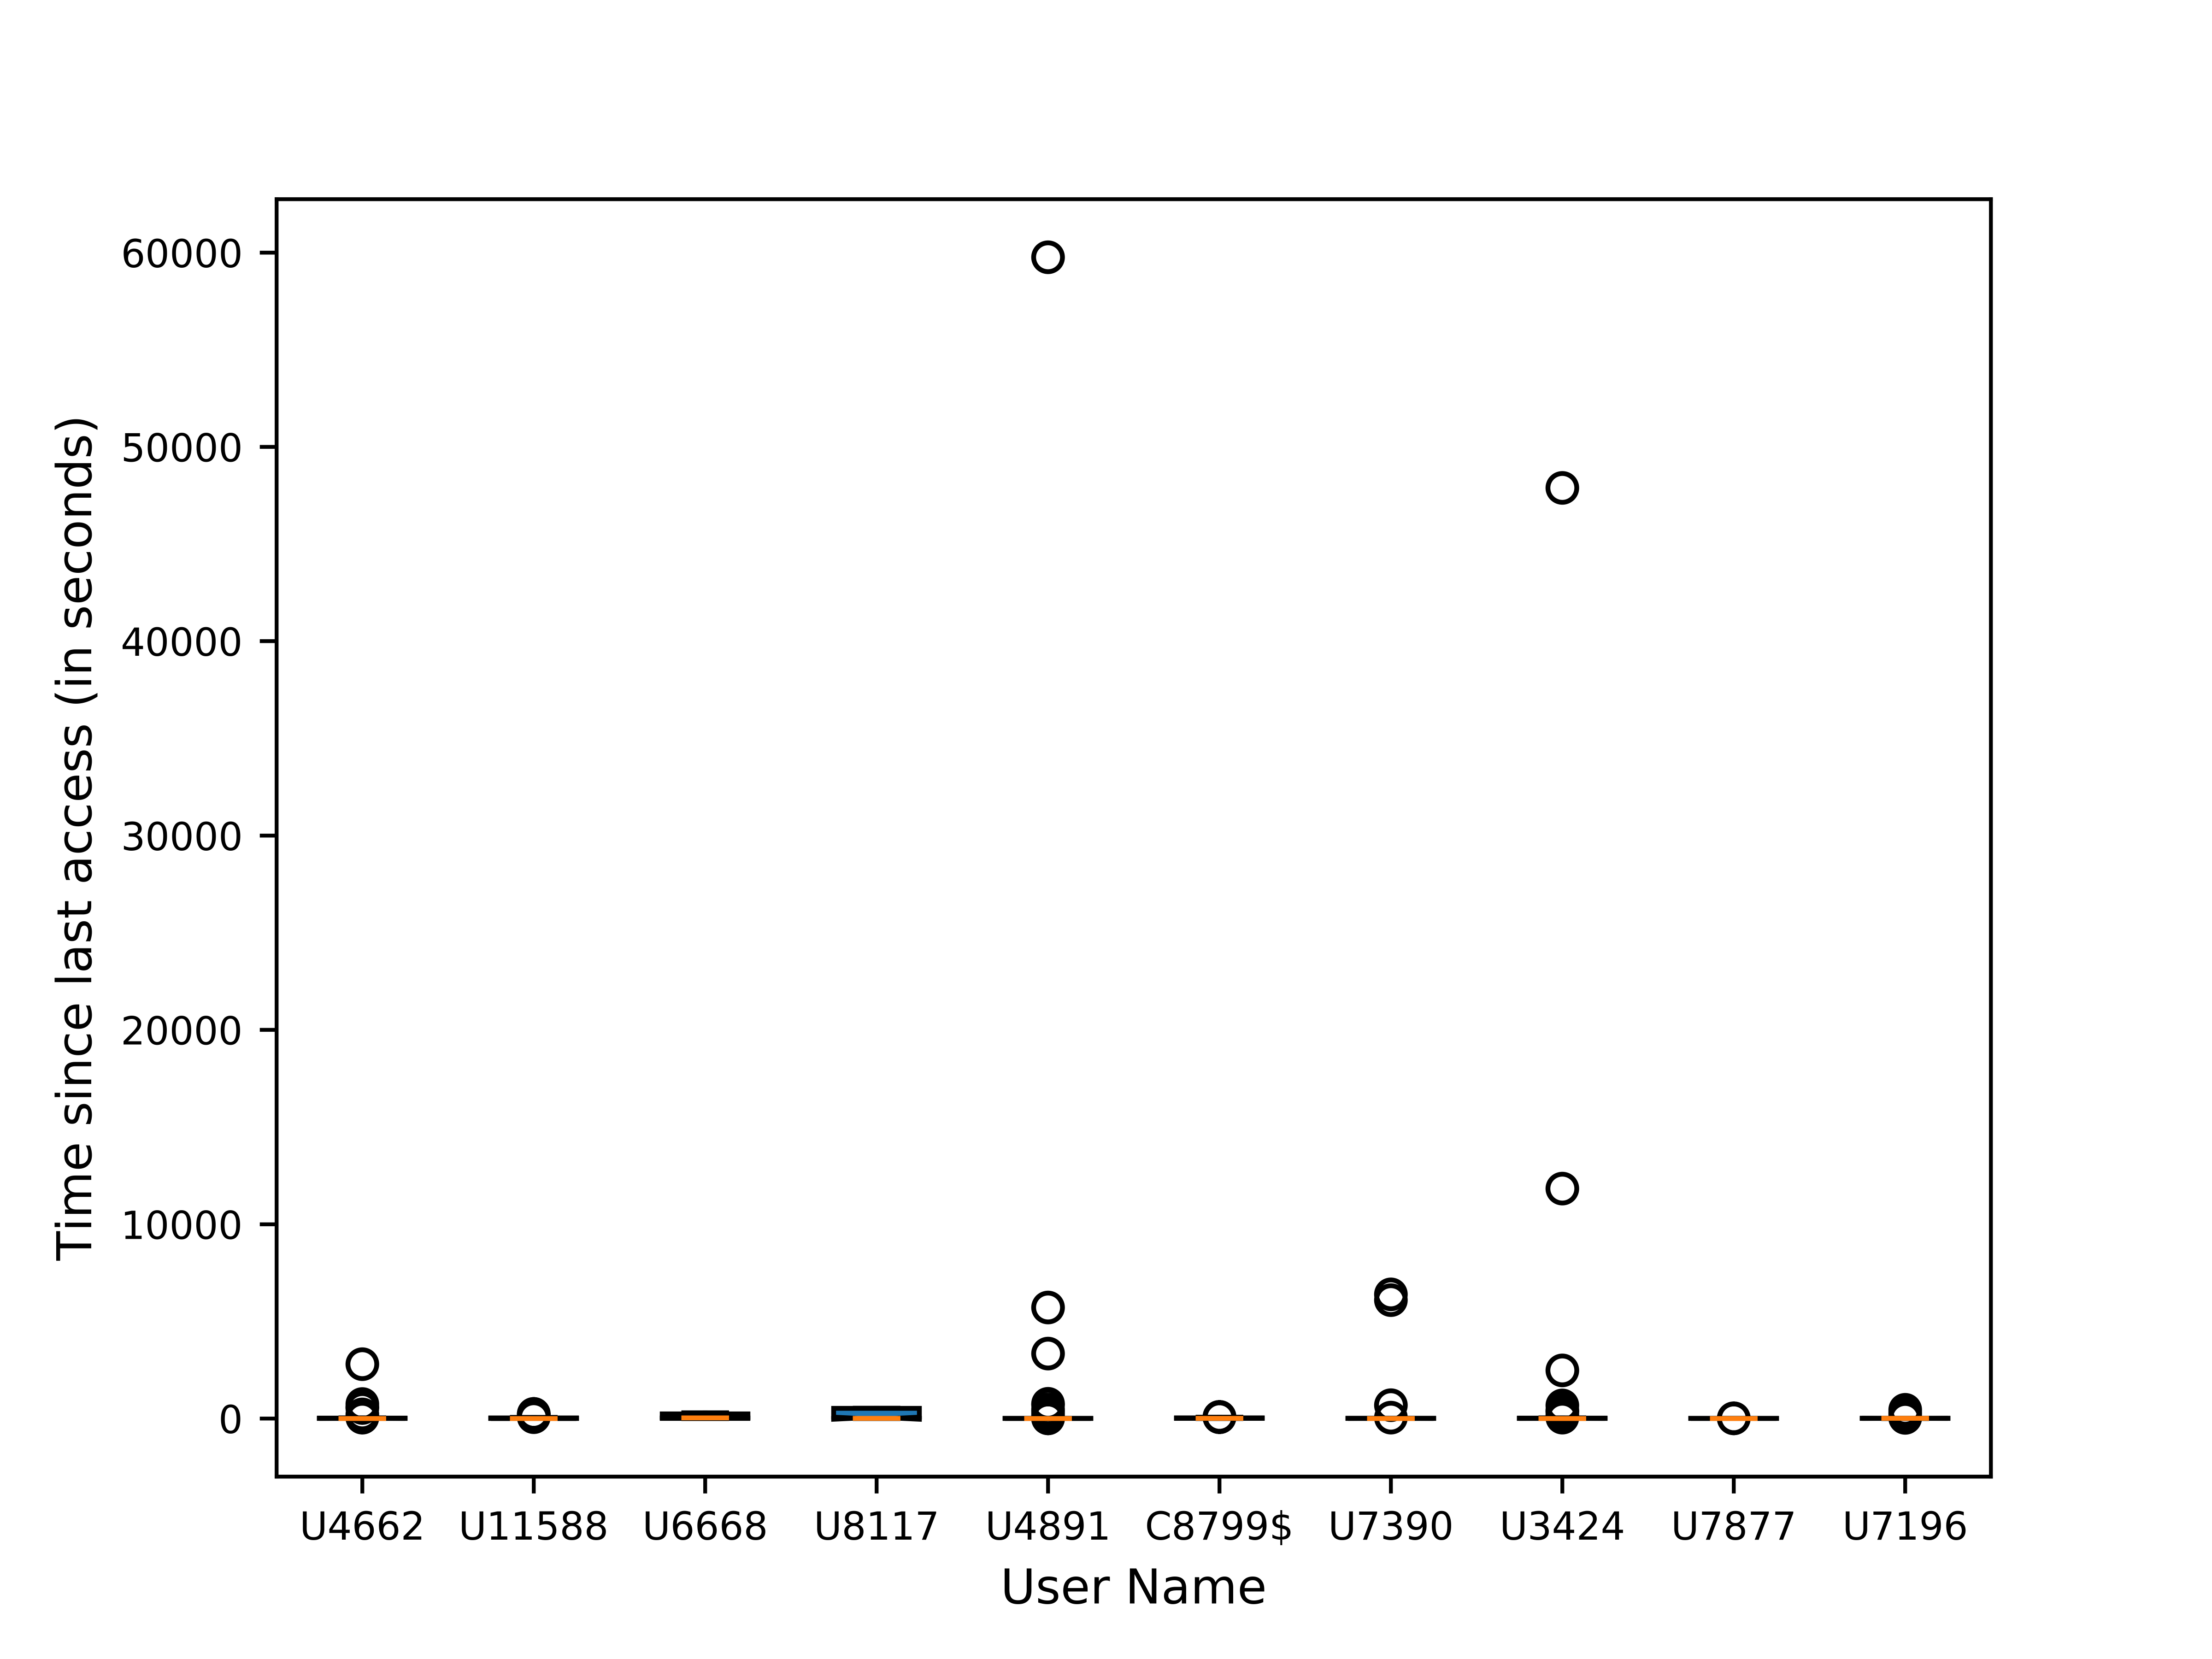
\includegraphics[scale=1.6]{evaluation/highest_offender_time_since_last_access}
	\end{center}
	\caption{The top 10 highest offenders' seconds since last access.~\label{fig:time_since_last_access}}
\end{figure}

Focussing on the highest offending users allows us to see more clearly why the network thought certain users were deemed anomalies and whether the network may have been right.

Taking a look at the time since the last network access for the top 10 highest offending users in figure~\ref{fig:time_since_last_access} clearly shows that some very big deviations from users' times since their last network access. For example U4891 consistently has a very low time since last access, as can be seen from the box plot being very small and concentrated around that area. However there are some small and bigger deviations from this average, probably causing the network to flag them as suspicious.

\begin{table}[htbp]
	\centering
	\caption{The predicted features vs the actual features of the top offender (precision set to 2 decimals)}\label{tab:predicted_vs_actual_top}
	\begin{tabular}{lll}
		Label & Actual & Predicted \\ \midrule
		time\_since\_last\_access & 0 & 0.00 \\
		domains\_delta & 0 & 0.00 \\
		dest\_users\_delta & 0 & 0.00 \\
		src\_computers\_delta & 0 & 0.00 \\
		dest\_computers\_delta & 0 & 0.00 \\
		percentage\_failed\_logins & 0.0 & 0.00 \\
		success\_failure & 1 & 0.4 \\
		auth\_type\_0 & 1 & 0.1 \\
		auth\_type\_1 & 0 & 0.19 \\
		auth\_type\_2 & 0 & 0.00 \\
		auth\_type\_3 & 0 & 0.00 \\
		auth\_type\_4 & 0 & 0.00 \\
		auth\_type\_5 & 0 & 0.00 \\
		auth\_type\_6 & 0 & 0.00 \\
		auth\_type\_7 & 0 & 0.00 \\
		auth\_type\_8 & 0 & 0.00 \\
		auth\_type\_9 & 0 & 0.69 \\
		auth\_type\_10 & 0 & 0.01 \\
		logon\_type\_0 & 0 & 0.02 \\
		logon\_type\_1 & 0 & 0.00 \\
		logon\_type\_2 & 0 & 0.00 \\
		logon\_type\_3 & 0 & 0.00 \\
		logon\_type\_4 & 1 & 0.00 \\
		logon\_type\_5 & 0 & 0.05 \\
		logon\_type\_6 & 0 & 0.08 \\
		logon\_type\_7 & 0 & 0.08 \\
		logon\_type\_8 & 0 & 0.08 \\
		auth\_orientation\_0 & 0 & 0.58 \\
		auth\_orientation\_1 & 0 & 0.06 \\
		auth\_orientation\_2 & 0 & 0.00 \\
		auth\_orientation\_3 & 0 & 0.01 \\
		auth\_orientation\_4 & 0 & 0.00 \\
		auth\_orientation\_5 & 1 & 0.28
	\end{tabular}
\end{table}

\begin{table}[htbp]
	\centering
	\caption{The highest offending user's previous logins before the anomaly}\label{tab:prev_logins}
	\resizebox{\linewidth}{!}{
		\begin{tabular}{lllllllll}
			time & source user@domain & destination user@domain & source computer & destination computer & authentication type & logon type & authentication orientation & success/failure \\ \midrule
			212020000 & C14012\$@DOM1 & C14012\$@DOM1 & C14012 & C2106 & Network & LogOn & Success \\
			212020000 & C14012\$@DOM1 & C14012\$@DOM1 & C14012 & C2106 & Network & LogOn & Success \\
			212020000 & C14012\$@DOM1 & C14012\$@DOM1 & C2106 & C2106 & Network & LogOff & Success \\
			212023000 & C14012\$@DOM1 & C14012\$@DOM1 & C2106 & C2106 & Network & LogOff & Success \\
			212029000 & C14012\$@DOM1 & C14012\$@DOM1 & C2106 & C2106 & Network & LogOff & Success \\
			212043000 & C14012\$@DOM1 & C14012\$@DOM1 & C457 & C457 & Network & LogOff & Success \\
			212758000 & C14012\$@DOM1 & C14012\$@DOM1 & C14012 & C457 & Network & LogOn & Success \\
			212772000 & C14012\$@DOM1 & C14012\$@DOM1 & C457 & C457 & Network & LogOff & Success \\
			212784000 & C14012\$@DOM1 & C14012\$@DOM1 & C14012 & C457 & Network & LogOn & Success \\
			212797000 & C14012\$@DOM1 & C14012\$@DOM1 & C457 & C457 & Network & LogOff & Success \\
			213233000 & C14012\$@DOM1 & U6147@DOM1 & C14012 & C14012 & Unlock & LogOn & Success \\
			213233000 & C14012\$@DOM1 & U6147@DOM1 & C1521 & C14012 & Unlock & LogOn & Success \\
			213657000 & C14012\$@DOM1 & C14012\$@DOM1 & C14012 & C457 & Network & LogOn & Success \\
			213671000 & C14012\$@DOM1 & C14012\$@DOM1 & C457 & C457 & Network & LogOff & Success \\
			213698000 & C14012\$@DOM1 & C14012\$@DOM1 & C14012 & C457 & Network & LogOn & Success \\
			213707000 & C14012\$@DOM1 & C14012\$@DOM1 & C457 & C457 & Network & LogOff & Success \\
			214557000 & C14012\$@DOM1 & C14012\$@DOM1 & C14012 & C457 & Network & LogOn & Success \\
			214571000 & C14012\$@DOM1 & C14012\$@DOM1 & C457 & C457 & Network & LogOff & Success \\
			214598000 & C14012\$@DOM1 & C14012\$@DOM1 & C14012 & C457 & Network & LogOn & Success \\
			214608000 & C14012\$@DOM1 & C14012\$@DOM1 & C457 & C457 & Network & LogOff & Success \\
			215457000 & C14012\$@DOM1 & C14012\$@DOM1 & C14012 & C457 & Network & LogOn & Success \\
			215471000 & C14012\$@DOM1 & C14012\$@DOM1 & C457 & C457 & Network & LogOff & Success \\
			215524000 & C14012\$@DOM1 & C14012\$@DOM1 & C14012 & C457 & Network & LogOn & Success \\
			215533000 & C14012\$@DOM1 & C14012\$@DOM1 & C457 & C457 & Network & LogOff & Success \\
			216357000 & C14012\$@DOM1 & C14012\$@DOM1 & C14012 & C457 & Network & LogOn & Success \\
			216371000 & C14012\$@DOM1 & C14012\$@DOM1 & C457 & C457 & Network & LogOff & Success \\
			216392000 & C14012\$@DOM1 & C14012\$@DOM1 & C14012 & C457 & Network & LogOn & Success \\
			216405000 & C14012\$@DOM1 & C14012\$@DOM1 & C457 & C457 & Network & LogOff & Success \\
			217145000 & C14012\$@DOM1 & C14012\$@DOM1 & C14012 & C2106 & Network & LogOn & Success \\
			217149000 & C14012\$@DOM1 & C14012\$@DOM1 & C2106 & C2106 & Network & LogOff & Success \\
			217257000 & C14012\$@DOM1 & C14012\$@DOM1 & C14012 & C457 & Network & LogOn & Success \\
			217271000 & C14012\$@DOM1 & C14012\$@DOM1 & C457 & C457 & Network & LogOff & Success
		\end{tabular}
	}
\end{table}

The highest offending action's predicted vs actual action are shown in Table~\ref{tab:predicted_vs_actual_top}. In this table (and following tables) features that are integers and not floats have been depicted as such, as all but the \(percentage\_failed\_logins\) features are integers. Any predictions made by the network are trimmed to 1 decimal point.

As can be seen the action itself isn't very weird, simply using a different method of authentication, a different method of logging in and a different authentication orientation. These methods themselves are not inherently anomalies, but the network learned that these actions are rarely made by the user, assigning a value of 0.0 to \(logon\_type\_4\) (interactive logon) and a value of 0.0 to \(auth\-type\_0\) (NTLM). When compared to the user's previous logins in Table~\ref{tab:prev_logins}, the last action really stands out as different. Many anomalies like this have been found. Often times the user logs in after a really long while or significantly changes their behavior by logging in using methods rarely or never used before. This signals that the network is doing a good job at recognizing the user's behavior and finding anything that deviates from it.